A través de un convenio de cooperación entre la Universidad Oberta de Catalunya y el Institut d'investigacions Biomèdiques August Pi i Sunyer (IDIBAPS), contamos con datos clínicos y de neuroimagen avanzada de personas que padecen esclerosis múltiple junto con un grupo control.

Como información clave para este estudio destacan las matrices simétricas de conectividad estructural. Estas matrices son el resultado del procesado de imágenes de \gls{drm}. Los índices obtenidos a través de estas técnicas, tales como las medidas del tensor, el número de fibras y el volumen de lesión pueden facilitar la obtención de medidas sensibles para diferenciar entre un paciente con un mejor o peor rendimiento cognitivo:

\begin{description}
 \item [\gls{dti}-\gls{fa}] Anisotropía fraccional
 \item [\gls{dti}-\gls{md}] Difusividad media
 \item [\gls{dti}-L1] Difusividad axial
 \item [\gls{dti}-RX] Difusividad radial
 \item [RAW] Número de fibras
 \item [LS] Volumen lesional
\end{description}

Los pacientes presentan un peor rendimiento cognitivo principalmente en atención y memoria. Para detectar una posible discapacidad cognitiva de los pacientes hemos realizado una evaluación neuropsicológica. Esta evaluación incluye una batería BRBN (Brief Repeatable Battery,  \cite{Boringa2001ThePractice}) junto con otras prueba cognitivas. Los dominios estudiados han sido los relacionados con aprendizaje y memoria. En la siguiente tabla podemos observar el número de pacientes cuya discapacidad está por debajo de puntuaciones -1 y -2 desviaciones estándares de una población de referencia (ver tabla \ref{table:totales}).

\begin{table}[h]
\centering
\begin{tabular}{|c|c|c|c|c|c|c|}
\hline
\textbf{Matriz/} & \textbf{Todos} & \textbf{HV} & \textbf{EM sim} & \textbf{Atención} & \textbf{Atención} & \textbf{Memoria} \\
\textbf{Grupo} &  & \textbf{(Sanos)} & \textbf{problema} & \textbf{} & \textbf{y memoria} & \textbf{} \\ \hline
\textbf{DTI\_FA}      & 140            & 42                  & 49                       & 14                & 16                          & 19               \\ \hline
\textbf{DTI\_L1}      & 140            & 42                  & 49                       & 14                & 16                          & 19               \\ \hline
\textbf{DTI\_MD}      & 140            & 42                  & 49                       & 14                & 16                          & 19               \\ \hline
\textbf{DTI\_RX}      & 140            & 42                  & 49                       & 14                & 16                          & 19               \\ \hline
\textbf{RAW}          & 211            & 42                  & 90                       & 29                & 21                          & 29               \\ \hline
\textbf{LS}           & 169            & 0                   & 90                       & 29                & 21                          & 29               \\ \hline
\textbf{TOTAL}        & 255            & 42                  & 101                      & 29                & 21                          & 32               \\ \hline
\end{tabular}
\label{table:totales}
\caption{Tabla con la distribución según clases cognitivas}

\end{table}

\section{Distribución de los datos}
\label{section:distdatos}

La información proveída por el grupo de Imagen Avanzada en enfermedades Neuroinmunológicas (ImaginEM) \cite{QueNeuroinmunologia} se encuentra organizada en una hoja de cálculo donde se presentan los datos clínicos de cada paciente anonimizado y una estructura en forma de distintos directorios donde se presentan cada matriz de adyacencia.

\subsection{Hoja de cálculo (Indice principal)}
La hoja del cálculo con los datos de cada paciente consta de 255 filas, una por paciente
y 33 columnas. Entre ellas se encuentra la columna $profile$ con los siguientes valores:

\begin{description}
\item [none] Persona con \gls{em} sin deficiencia cognitiva detectada.
\item [HV] Persona sin \gls{em}
\item [memory] Persona con \gls{em} y afectación en memoria
\item [attention] Persona con \gls{em} y afectación en atención.
\item [mem\_att] Persona con \gls{em} y deterioro cognitivo en memoria y atención.
\end{description}

\subsection{Directorios con matrices}
Estos directorios siguen un formato establecido donde cada fichero indica en su prefijo a qué paciente corresponde y, en función del directorio donde se encuentra, la medición de dónde proviene la matriz. Por ejemplo, el fichero situado en
\begin{lstlisting}
FIS/ADJACENCY_MATRICES_GRAPH/DTI_indices/FA/FIS_001_FA.csv
\end{lstlisting}
corresponde con la medida DTI-\gls{fa} del paciente de cuyo identificador es FIS\_001. En la tabla de la imagen \ref{figure:rutas} se describe detalladamente esta estructura.

Cada fichero que contiene los valores de una matriz está almacenado en formato \gls{csv} conteniendo todos ellos 76 filas y 76 columnas sin ningún valor nulo o vacío.

\begin{figure}[H]
\centering
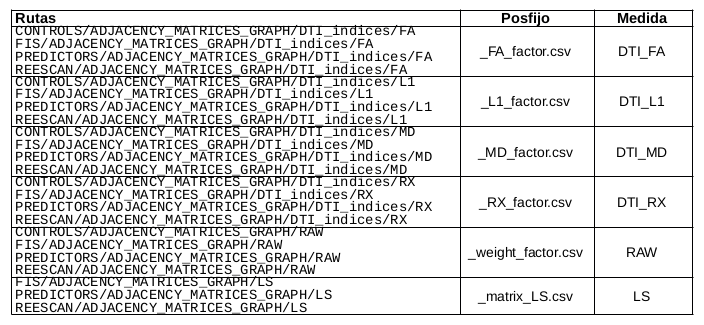
\includegraphics[width=1\textwidth]{figs/datos/rutas.png}
\caption{Imagen con la tabla de los directorios de matrices y sus medidas correspondientes}
\label{figure:rutas}
\end{figure}

\section{Características de los datos}
Para cada instancia que disponemos de los datos, contamos con seis matrices de adyacencia de tamaño $76 x 76$. Aparte de estas matrices los valores de estas matrices, de la hoja de cálculo se presentan 33 columnas. Es decir, disponemos ejemplares de la muestra con hasta $76 x 76 x 6 + 33 = 34689$ atributos cada uno. 

Los valores de las matrices son completos, es decir, si una instancia tiene una matriz, todos sus valores están presentes. Como se ve en la tabla \ref{table:totales}, no todas las instancias tienen todas sus matrices. Por otra parte, también se encuentran 40 matrices ``perdidas'', sin correspondencia con ninguna instancia de la hoja de cálculo y, por lo tanto, descartadas para el estudio. 
